We have chosen an (almost standard-conform) UML-class diagram notation.  (cf.
Figure~\ref{fig:classdiagram}).


\begin{figure}[htbp]
  \centering
  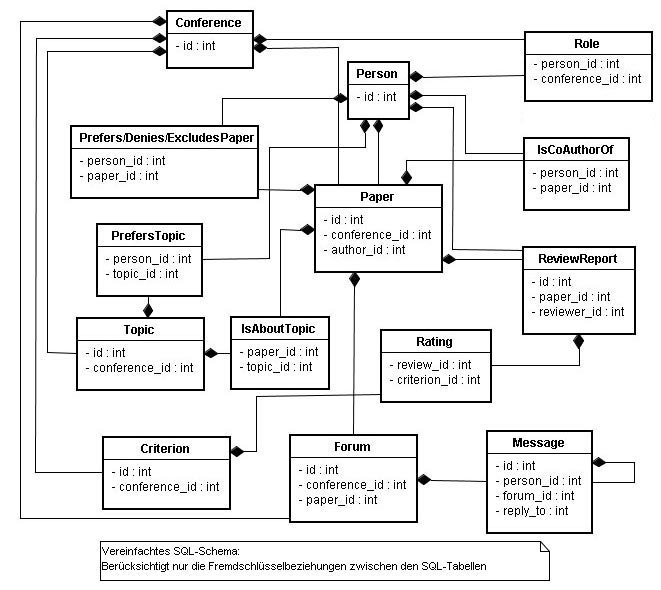
\includegraphics[height=12cm]{../sql/db_schema}
  \caption{Class diagram}
  \label{fig:classdiagram}
\end{figure}

The diagram was worked out after discussion on the bulletin board in the
plenum. It took inspiration from the two specification deliverables
\cite{coma:spec1} \cite{coma:spec2}, at least the static part, for instance
the ER-diagram from \cite{coma:spec1}, but also from different variations
from the data model of this document, version 2.

The graphical representation from Figure~\ref{fig:classdiagram} is
simplified insofar as plain fields are left out. Those are specified in
more detail





\subsection*{SQL-model}
\label{sec:datamodel.sql}
%

The following is as ``textual'' representation of the data model, as worked
out by S. Esquivel, M.\ Albari, G. Biederbeck, and others.


\lstinputlisting[basicstyle=\scriptsize]{../sql/db_schema.txt}


\iffalse
I leave out in the discussion of the ``central'' classes as they seems
obvious, but concentrate more on the tables reprasenting classes.



\subsubsection*{Role and Roles}
\label{sec:roleandroles}%

Deviating from the picture on the blackboard (and from
Figure~\ref{fig:classdiagram}), there are \emph{two} tables: \texttt{Role}
and \texttt{Roles}. This is introduces to model the fact that \emph{the
  same person} can be present in \emph{two} conferences at the same time in
two different ways\footnote{Remember: that was not on the plate in the
  original Version 2 of the doc. In the older model, a person was
  associated with exactly one conference.}


\subsubsection{Preferred topics}
\label{sec:preferredtopic}











%\newpage
\fi


\iffalse
\begin{figure}[htbp]
  \centering
  \includegraphics[height=12cm,angle=90]{../figures/data-model}
  \caption{Class diagram}
  \label{fig:classdiagram}
\end{figure}
\fi


\iffalse
We start deconstructing the diagram according to the classes, obvious
fields we omit in the discussion here (they might get filled in later). We
start with the main ``entities'', and discuss the ``associations'' later.


\begin{table}[htbp]
  \centering
  \begin{tabular}[t]{ll}
    Conference &
  \end{tabular}
\end{table}
\fi








\newpage


\subsubsection{SQL-Spec}
\label{sec:sql}
\lstset{basicstyle=\scriptsize,numbers=left,numberstyle=\tiny,stepnumber=5,language=sql}

Relevant is only the SQL-Spec.




\lstinputlisting[caption=DB: conference,label=code:sql.conference,firstline=27,lastline=44]{../sql/db_schema.sql}%


The table conferences (cf.\ Listing~\ref{code:sql.conference}) contains all
the conferences being hosted by the server. We propose that there exists as
\emph{default, empty conference} to begin with as entry in the table. This
default conference is charakterized by the empty string. Most of the
entries in the table should be self-explanatory. For the deadlines, the
following ones are foreseen, in the order of events:
\begin{enumerate}
\item The \emph{abstract submission deadline.} This typically is a
  (secondary) deadline for \emph{authors} shortly before the paper
  submission deadline.  It allows the authors to upload an abstract of
  their papers. There is not much ``semantics'' behind this deadline, only
  that experience shows that it helps in organizing the conference to know
  in advances how many papers there will be, about what topics etc. A
  further advantage of the abstract submission deadline is that it may
  ``encourage'' the authors to try to meet the real paper deadline a little
\item The \emph{paper submission deadline.} This is the most important
  deadline for authors, namely: when must they finished their work! After
  that deadline, no new papers or new versions of the paper may be
  uploaded.\footnote{A exception may be, that the chair make a personal
    exception or something, but that's only by circumventing the normal
    process.}
\item The \emph{review deadline:} That's the first deadline for the
  \emph{reviewers,} namely: when must they have finished their reading job
  and must have handed in the grades; on the basis of this information, the
  discussion and selection starts.
\item The \emph{notification deadline:} this is the deadline when the
  \emph{selection} has ended and when the authors are notified about their
  success or failure.
\item The \emph{final version} deadline: afterwards, the successful authors
  may be required to up-load the ``very final version'' to be printed,
  sometimes also called \emph{camera ready version}, which takes into
  account the criticism of the reviewers.
\end{enumerate}


\medskip{}



The \emph{persons} using the tool are all kept in the table
\texttt{Person}. Again most fields should be self-explanatory. Not all
fields of a person must be filled in; in order to facilitate communication,
we require the \emph{email address}; for secure identification furthermore
a password (cf.\ Listing~\ref{code:sql.person}).  An

\lstinputlisting[caption=Person,label=code:sql.person,firstline=45,lastline=60]{../sql/db_schema.sql}%

\medskip{}

Crucial for the interaction of persons with he tool are the \emph{roles}
the persons play (cf~\ref{code.sql.role}. Some of them were mentioned
informally in the requirements specification \cite{coma:requirements}. In
the course of the semester, we reached at \emph{no agreement} how to
represent the role. Thus, neither the representation no the exact choice of
roles are indicated in the shown SQL-code. 

\lstinputlisting[caption=Role,label=code:sql.role,firstline=65,lastline=79]{../sql/db_schema.sql}%


In the textual representation which is agreed upon as supplementary global
spec, we fixed the roles of Table~\ref{tab:roles} to be mandatory. The
numbers indicate the numerical representation, if no enumeration and
additional table \texttt{Roles} is chosen.

\begin{table}[htbp]
  \centering
  \begin{tabular}{lll}
    \\
    role & integer
    \\\hline
    without role & 00 
    \\
    admin & 01
    \\
    chair & 02
    \\
    reviewer & 03
    \\
    author & 04
    \\
    participant & 05
    \\
  \end{tabular}
  \caption{roles}
  \label{tab:roles}
\end{table}



%


\begin{abstract}
  This document (at the current stage) descibes the data that are to be
  represented in the Tool.  \ifweb It is available also as
  \href{main.pdf}{pdf}.  \else It is also available via the website. \fi It
  is not the full specification, in particular, no dynamic behavior is yet
  represented or described (except by some hints)
  
  It serves to \emph{consolidate} at least this core part and allow to push
  ahead, in particular the SQL-group.  It is considered
  \emph{consolidated}, in that is is final up-to necessary changes.  To
  reflect the development, the specification is qualified with a versioning
  number.
  
  The document does not yet mention yet all the restrictions, the dynamic
  apsects, or the scenarios and phases and further information that has
  been found in the specifications generated in the first phase.

  \noindent
  \textbf{version:} \version\  (\verb+$Id$+)
  \\
  \textbf{status:} \status
\end{abstract}



%%% Local Variables: 
%%% mode: latex
%%% TeX-master: "main"
%%% End: 

%\tableofcontents{}


%\section{Introduction}
\label{sec:introduction}




The document describes \emph{informally,} i.e., in plain English, the
functionality (plus rather the purpose) of \Coma, a tool to assist in the
distributed preparation, organization, and processing of a conference,
workshop, or similar event.

The rest of the document sketches the intention of the project, the
informal functionality etc. We are not explicit about specific technologies
or how to realize the task.


\iffalse

As we intend to start \emph{early} with the \emph{integration}, the
required methods should be provided rather quickly without being (fully)
implemented (i.e., as \textit{stubs}). See also the time-line of the
project.

We provide as starting point a first implementation of the abstract syntax
(cf.\ Section~\ref{sec:abstractsyntax}) and a small textual printer in the
utilities package.



If from the perspective of a package, changes or extensions seem necessary
or desirable as far as the abstract syntax is concerned, the wish should be
uttered and justified as early as possible to all participants (and then
potentially implemented by us or the requester, if everyone agrees).

\fi




\subsection{General purpose}
\label{sec:purpose}

Scientific conferences nowadays are in general prepared, advertised, and
managed via the web. In particular, part of the organization is done in a
``distributed'' and loosely coupled manner, i.e., the actors in the
organization work at various locations, time zones, etc.

At an rather abstract level, the goal is to allow a group of experts, to
collaborate to find an agreement in selecting from a set of contributions
to the conference.






\section{Represented data}

Since this part is the best specified, we start the description here. This
is not intended as concrete data model (let alone SQL-code), but describes
in general terms, what is in the range of the tool and what not. There are,
of course, links with the data model.





\subsection{Users}
\label{sec:users}


By \emph{users,} we mean people interacting with the service. More
precisely, users are those people which are represented and modelled in one
form or the other inside the tool, which is to say, some accidental surfer
is not user. Users interact in various roles. The role can change over the
\emph{time} and the role may differ in differente conferences.

The roles supported by \Coma\ are
\begin{description}
\item[administrator:] The administrator is not part of the scientific
  organization of the conference, i.e., he does not take part in
  \emph{semantical} decisions concerning the content. 
\item[chair:] program committee chair (\emph{chair} for short). There might
  be more than one chair. He or she is chairing the program committee and
  is therefore part of the committee. A chair is in some sense the
  ``dictator'' concerning semantical issues which means he is granted more
  privileges than the others.\footnote{Whether it's wise to act as a
    dictator, overruling all the others in the committee, taking lonely
    decisions, or undoing decisions taken in consensus is a different
    question and outside the possibility of our modeling.} Basically he
  can change all data all the time, for instance, he can remove or add
  people from the committee, throw out papers, etc. Again, whether it's
  smart to do so excessively is another question, but sometimes his
  intervention is necessary. A simple example: one of the reviewers does
  not do his work (for instance does not read the assigned papers), the
  chairman must be able to throw him out, which means for the tool: remove
  him from the data-base etc.\footnote{Note that those semantical changes
    of the chair are different from what the administrator could do. The
    chair should be able to make the changes \emph{within} the software,
    while the admin in some sense is outside. The admin can probably also
    change data, for instance by directly querying the data base (or wiping
    out the data base from the file system, for that matter \ldots) but
    that's something else.}
\item[reviewer:] = program committee member
\item[author:] each paper must have at least one author, but there might be
  more. For the software, one author plays are more important role than the
  others, namely the one who interacts with the organizers. This is the
  \textbf{corresponding author}.
\item[participant] of the conference, i.e., a person who attend the
  conference and listens to the presentations etc.
\end{description}

Each user should be identified uniquely, which means, identities are shared
(or at least are shareable) between conferences.


\subsection{Restrictions and side conditions}
\label{sec:restrictions}


The groups of people are not disjoint, in other words, an individual can
interact with the service in different roles (at different times).  Crucial
is to obey certain \emph{rules} concerning who (respectively who in which
role) is allowed to do what or to see what. This also changes during time.

Here is a number of informal restrictions.

\begin{enumerate}
\item a not-yet-accepted paper may only be seen by the author who submitted
  it.
\item the identities of submitting authors must be unknown to the outside
  and also among the authors themselves
\item a reviewer must not review his own paper, i.e., he must of course not
  influence the decision
\item an author never sees the discussion on his paper
\item an author never sees the identity of his reviewers
\item an author sees the verdict once all decisions are taken
\item a reviewer does not see the reviews of his colleagues, until he has
  sent his own review
\item a chair can see everything all the time.
\item it is expected that at least one author of an accepted paper
  participates at the conference, i.e., each accepted paper must be
  presented by an author
\item \emph{optional:} a reviewer must not know the identity of the authors
  of the papers he reviews. This is also known as \emph{double-blind}
  review.
\end{enumerate}







\section{Phases and events}
\label{sec:phases}%

The organization of the conference takes a limited amount of time, which is
fixed at the beginning. We distinguish the following main phases:
\begin{enumerate}
\item assembly
\item paper submission
\item reviewing, consensus finding about the selection of the submission
\item registration
\end{enumerate}

The phases themselves are ordered linearly, the exact duration or distance
of the single events should be adaptable. In the following, we discuss the
purpose of the phases the outcome of each. Most (but not all) phases are
separated by events.


\medskip



\iffalse
\paragraph{A word of warning} 
The following phases reflect an idealized situation, where all phases are
cleanly separated, all actors in the game do the correct things etc.
Sometimes this will not be the case. Clearly, a user must be able to
correct information he provided; one instance is described in
Section~\ref{sec:submission}, where a submission is replaced by a newer
one. 
\fi










\subsection{Event: Configuration}
\label{sec:configuration}
%%

Configuration serves a rather simple goal, namely the preparation and setup
for the rest of the phases. After installation, its includes to fix basic
data of the conference, which means it's name, it acronym, the date (begin
and end) and the location of the conference. Furthermore, the chairs of the
program committee are (probably) known.






\subsection{Phase: Assembly}
\label{sec:assembly}

The assembly is done by the \emph{program chairs.} The result of the
assembly phase is the \emph{program committee,} i.e., the collection of
experts or individuals that will, in later phases, decide about the
program.

The program committee is not \emph{self-assembled.} It is the task of the
program committee to \emph{invite} members via email.

Invitees are free to decide, whether they wish to participate, which means
they should actively \emph{acknowledge} participation or they should
reject. Before they acknowledge, they are called program committee
candidates, or \emph{candidates} for short. By default, candidates are not
members unless they positively acknowledge participation.  They can
register with the committee by using a web-interface. By acknowledging,
they also fill in further relevant personal data, such as affiliation
(=professional address), full name, preferred email address, home page.



\subsection{Event/document: Call for papers}
\label{sec:cfpapers}

Once the program committee is fixed the conference is ``advertised'', i.e.,
authors are invited to contribute to the event. The document, basically an
url i.e., the ``web-page'' which contains this advertisement is called the
\emph{call for papers}. It must announce all information about the
conference relevant for authors, which

\begin{enumerate}
\item basic conference data
  \begin{itemize}
  \item date
  \item name, acronym
  \item location
  \end{itemize}
\item important dates for authors
  \begin{itemize}
  \item optional: deadline for abstracts
  \item deadline for submission (cf.\ Section~\ref{sec:deadline})
  \item notification date (cf.\ Section~\ref{sec:notification})
  \item date for the final, i.e., a possibly corrected version of the
    paper.


  \end{itemize}
\item reference to the submission page
\item short description as free form text
\item names, affiliations and perhaps other information about the
  organizing people.
\end{enumerate}



\subsection{Phase: submission}
\label{sec:submission}

The effect of the announcement is that authors decide to contribute to the
conference. The contributions are called \emph{papers.} The paper is
\emph{uploaded} by an author onto the appropriate web page, the act of doing
so is the \emph{submission.} 

A paper has at least one \emph{author,} but may have more than one.  One
author may have more than one paper. One author of a paper is considered as
the main author, known as the \emph{corresponding author}. This is the
author the organization of the conference deals with. 

An author can decide to \emph{retract} a paper. In this case, no older
versions (if any) of the paper are restored, but the paper is removed
completely.





\subsection{Event: submission deadline}
\label{sec:deadline}

The submission phase is terminated by the \emph{submission deadline,} a
pre-announced time after which no submission is possible. Until that time
an author can submit many versions of the same paper. Only the last one
before the deadline counts, i.e., each later version overwrites the earlier
one.\footnote{We cannot prevent that an author acts stupid and submits a
  later version of the same paper erroneously as a new paper, because we
  cannot check the semantics of the paper.}

It is possible for an author to remove a paper even after the deadline (see
Section~\ref{sec:submission}).



\subsection{Phase: Reviewing}
\label{sec:reviewing}

Reviewing is the process of selecting from the submission a set of papers.
The selection is done by the program committee in a joint effort using the
web server. The (informal and conflicting) goals are:
\begin{description}
\item[quality of paper selection:] Since in general there are more papers
  than time on the conference, the best papers are to be selected.
\item[load balance for reviewers:] In order to form an opinion about a
  paper, a reviewer must read and understand it.  This workload must be
  distributed in a fair manner for the members.
\item[load balance for papers:] Each paper gets (in general) more than one
  reviewer, to make the decision less random. Each paper should get an
  equal share of the reviewing task.
\item[quality of reviewer selection:] Each reviewer gets the papers that he
  wants to and/or he is the best expert for.
\end{description}

The above specification obviously is informal and unprecise as it allows a
number of interpretations. We do not fix an exact specification here,
because there are probably many plausible solutions.  Instead we discuss
aspects of the mentioned goals. In the specification task, we would like
more explicit proposals to solve this problem.

\subsubsection{Assignment of papers}

One task is the \emph{assignment} of papers to reviewers. It is to be
expected that there are more papers than reviewers, and furthermore one
should cater for the case that each paper gets more than one reviewer.
Preferably, and unlike the selection of the papers, the assignment is done
\emph{automatically,} i.e., without general discussion.

Furthermore, the assignment should be ``fair'' wrt. the reviewers and wrt.
the papers, in that the \emph{load} is equally shared. An easy and not very
useful solution would be to make a random assignment, under the side
condition of approximate load balance. The disadvantage is that, in
general, the members of the committee have slightly different fields of
expertise, and preferably a member evaluates papers in a field he is a
strong expert of. % Two (at least) could be imagined.

\begin{description}
\item[Assignment by topic] Papers are classified according to a finite list
  of \emph{topics.} The topics are predefined for the conference, and the
  \emph{author} must pick those he feels his paper fits in. He might choose
  more than just one topic. Also each reviewer, beforehand, chooses a
  number of topics which he prefers to read papers from. Once the papers
  are in, the software tries to take the preferences of the reviewers into
  account, but of course still maintaining load balance concerning the
  numbers of papers per reviews and the numbers of reviewers per paper
\item[Assignment by paper] This approach does not rely on predefined
  topics.\footnote{This does not mean that there could not be predefined
    topics.} Each referee shortly looks at the list of papers and declares
  preferences (or dislikes) according to some schema. It this might be very
  simple like ``I want 2, 17, and 42''. Also, it should be possible to
  state: ``I cannot review this paper.''.\footnote{Typically this is the
    case, if one sees that it's a paper by some friend/colleague \ldots so
    that one fears that one does not have an unbiased opinion.} Again in
  this scheme, the selection mechanism should take the choices into
  account, but adhering to the side condition of balance. In other words:
  if someone only picks one paper, it does not mean he will get only one.
  If 15 people find paper 76 very interesting, it does not mean that paper
  76 gets 15 reviewers.
\end{description}


One can imagine to combine those approaches, or to make it a chooseable
alternative.

\subsubsection{Selection of  papers}
\label{sec:bestpapers}%

In general there are more papers than there's time, so the intention is, of
course, to pick the best of them.  To talk about finding the ``best
papers'' is misleading, though, because this uses the idealistic assumption
that there are best papers and one just does not know yet which ones they
are. On the other hand: even if it is more than questionable whether there
is a globally and universal quality scale to be applicable to the papers,
it does not mean that some papers are better than others, in the sense that
most everyone would agree on that. The task is to come fast and efficiently
to an agreement about this issue.

\medskip


Let's assume two fundamentalistic approaches, which sheds light about the
range of possibilities. Both sketched approaches are in practice not very
useful and should be avoided.  In order to talk about the best papers, one
obviously assumes an (imaginary) \emph{linear order} which needs to be
determined by consensus and now the question is, how to reach this order.

\begin{description}
\item[Discuss everything] One standpoint is: all participants discuss all
  papers in a free-form manner until all agree on some order, and this
  fixes the best papers. This solution is impractical: A \emph{rational}
  agreement, i.e., an agreement based on common understanding, would
  require that all reviewers read all papers (which one wants to avoid
  \ldots). And even if all papers are read and discussed by all committee
  members, to reach at a common order lead to endless dispute.
\item[Discuss nothing] The opposite standpoint is: There is \emph{no
    discussion} at all. Each reviewer gives the paper(s) he reviews a
  numerical value, say a mark. At the end the marks for each paper are
  averaged,\footnote{In general a paper gets reviewed by more than one
    expert.} the results are ordered linearly, and then the best are
  chosen.\footnote{For the discussion we ignore the fact that there might
    be equal outcomes.} That is the most efficient solution but it might
  easily lead to bad decisions. In general, there is more than one reviewer
  per paper but there are in most cases not more than 4, and this makes the
  mean value of ratings rather random.
\end{description}

\medskip

As perhaps from the discussion, there will not be a clean, mathematically
optimal solution for the problem; basically the decision finding requires
human intelligence and social interaction. The trick will be to
\emph{assist} in this social process, to make it more efficient than free
discussion but more rational than random selection.




\paragraph{Possible states}
\label{sec:possiblestates}

Next we discuss which general states a paper can have during the reviewing
phase. \emph{Ultimately,} the judgment for each paper will be:
``\emph{accepted}'' or ``\emph{rejected}'', which is when all the papers
are decided. A proposal for a schema of states could be:
\begin{displaymath}
  \begin{array}[rcl]{rcl}
    \mathsf{status} & \bnfdef & \mathsf{decided} \bnfbar \mathsf{undecided}
    \\
    \mathsf{decided} & \bnfdef & \mathsf{accepted} \bnfbar \mathsf{rejected}
    \\
    \mathsf{undecided} & \bnfdef & \mathsf{unreviewed} \bnfbar \mathsf{unclear}
    \\
    \mathsf{unclear}  & \bnfdef & \mathsf{conflict}  \bnfbar \mathsf{inconclusive}
  \end{array}
\end{displaymath}

There, a paper is yet undecided if it's not yet reviewed or the situation
is unclear. Two causes are that there is a serious disagreement about the
quality. For instance if one reviewer thinks the is very good in one
category, and another one says it's very bad in the same category, this is
an indication that one better looks at this point again. One could
distinguish from that a situation where a paper is in the
``so-la-la''-range. In general, most submissions are in the middle-field.
In this case there might not be enough statistical evidence to distinguish
between two contributions with slightly different ratings.




\paragraph{Decision herding}

The core of a solution is to \emph{focus} the process. Certain discussion
is unavoidable/wanted, but the participants should focus (or rather helped
to be able to focus) on the right, i.e., discussion-worthy things. Since
the goal of the discussion is to find an agreement, discussion-worthy
things, in first approximation, are those which are not yet decided.

Basically, the ones taking part in the discussion, must be assisted to get
a good overview of the status of the debate and what things profitably to
do next. This includes some form of \emph{visualization} (which might be as
simple as a table) of relevant information. Relevant information could
include:

\begin{description}
\item[per reviewer:] A reviewer will (if not ``forced'' otherwise)
  concentrate on ``his'' papers perhaps his reviews.  So he should be
  presented ``his'' part of the task first. If not restricted, he might of
  course look also at other parts/aspects of the information.
\item[``executive info'':] short, high-level overview over the status and
  progress (how many papers are decided, how many still to be discussed.)
\item[delays:] Indication about missed deadlines (someone has not yet send
  his reports or similar)
\item[chosen focus:] Some papers are chosen (for instance by the chair) to
  be discussed next.
\end{description}

Of course, the access to the information must obey the restrictions
concerning the various user groups mentioned in
Section~\ref{sec:restrictions}.






\paragraph{Criteria}
\label{sec:criteria}

As said before, the reviewers study the paper to come to an opinion about
the quality of the contribution. In general one does not wish (only) a
uniform single numerical value, but a (reasoned) rating in various
categories. Those categories could include


\begin{description}
\item[overal rating:] A single numerical value which expresses the overall
  quality of the paper, taking all aspects into account
\item[originality:] how new is the result/content?
\item[soundness:] Is the technical content sound or are there serious
  errors in the argumentation/proofs/results \ldots
\item[relevance:] how good does the paper fit into the theme of the conference
\item[style:] How well is the paper written? How sloppy is it? Is the
  English (or German \ldots) ok?
\item[confidence:] How confident is the reviewer about his own opinions?
  This depends on whether he understood most of it, whether he considers
  himself an expert in the topic etc.
\end{description}

The list should be adaptable per conference, but the above could be taken
as \emph{default.}





\subsection{Event: Notification}
\label{sec:notification}


\emph{Notification} is the event which informs the authors about the final
decision of the reviewing process. There are only two possible outcomes,
namely \emph{yes} or \emph{no} for each paper. Besides the binary decision,
the author is informed about the ``opinion'' concerning his submission.
Concerning what information the authors are allowed to see, cf.\ also
Section~\ref{sec:users}.

\subsection{Event/document: Call for participation}
\label{sec:cfparticipation}%

As the call for papers (cf.\ Section \ref{sec:cfpapers}), the call for
participation is basically an advertisement. This time the addressees are
not the potential authors, but potential participants of the conference
itself. The call for participation contains similar information about the
conference, but as additional information of course the program, i.e.,
the list of accepted papers with authors etc.






\subsection{Phase: registration}
\label{sec:registration}

This phase is characterized by the interaction of \emph{participants} of
the conference with the tool. Users can register with the conference, i.e.,
announce their participation. Again this will be done via some interface.
The registration should be acknowledged.  

The participant provides the usual personal information (name, title,
affiliation). Furthermore, he is offered a number of options he must choose
from:
\begin{itemize}
\item in which role he registers: as student (reduced fee) or as full
  participant
\item preferred method of payment (+ credit card info, if applicable)
\item dietary restrictions (vegetarian, etc)
\end{itemize}

Furthermore, if a user registers before a predefined deadline
(\emph{``early registration''}), the fee is reduced.














\section{Further requirements}
\label{sec:further}

In this section, we list some further requirements, which are not so much
functional specification, but rather general requirements or also 


\subsection{Adaptability, parameterization, and options and defaults}
\label{sec:adaptability}%

Since the intention is that the tool is not usable for just one conference,
but for many, certain things must be adaptable per conference. We call one
conference an \emph{instance} of a conference.  Each instance of a
conference is characterized by number of basic data, which must be provided
in the configuration phase. At later phases, additional information
(papers, reviewers etc.) are provided.

All in all, the whole thing is required to offer quite an amount of things
the users can \emph{adapt}. Part of these adaptability is described and
discussed here and is part of the standard scenario of reviewing. There are
much more things imaginable, for instance: besides the program chair,
someone wishes to have a financial chair and a local organizer listed on
the web-page, someone things the background color of the generated
web-pages should be green, and weirder things \ldots).

To make the tool useful in practice, a good balance between hard-coded
decisions and adaptable variations will be crucial. A couple of things
should be kept in mind here:
\begin{description}
\item[Modesty:] don't get carried away! The fact that one can easily
  include another battery of check-buttons to adapt this and than and other
  does not mean the user will like this. 
\item[Empty options/switching off features] take care that options or
  features can also be switched off. If the user don't want a requistration
  phase in the, he may completely switch it off, for instance. This is
  related also to the point ``modesty''.
\end{description}

A useful technique in this context is also the choice of \emph{good
  defaults.} There are always users, who want to fiddle with everything and
they should be given freedom to a certain extent. There are also others,
who don't bother, \emph{provided} the default setting are usable.
Therefore, making good defaults enhance and keep the number of necessary
variation points beyond that small, enhances the usability quite a lot.








\subsection{Webserver \& download version}
\label{sec:uses}


The software should be usable also as some web server managing more than
one conference. The alternative is, that one user (in the role of the
admin) downloads the source code, install it, adapts it for his or her
needs and uses it for organization.  The consequence of the ``webserver''
requirement is simple: more than one conference must be held in the data
base at the same time, without any information flow (other than the
information concerning the general public and other than by the
administrator) between the two conferences.\footnote{Actually, the download
  version is more challenging in some sense, it has higher requirements on
  platform independence and easy installation. The webserver can be
  installed and ``massaged'' by the experienced admin until it runs
  stable and then rot.}




\subsection{Changeability, non-standard scenarios}

A general remark which applies to almost everything described above.
namely: we concentrated on the smooth, standard evolution of the event.

In general, the tool must be prepared that this is not the case, which
basically means, that choices once made must be \emph{changeable.}
Basically, all data in the data base must be ``manually'' adapted if need
be, the problem is that is must not unnecessarily interfere with the
process. Possible non-default scenarios are:
\begin{itemize}
\item a reviewer does not review, and is removed.
\item an additional review about a paper is delivered, or a paper is re-assigned.
\item the chair (or the committee) decides that one particular paper is
  rejected/accepted despite the fact that perhaps the numerical valuation
  or the status of the discussion would indicate otherwise. The valuation
  of the rest of the papers must not be ``confused'' by that.
\end{itemize}











%\subsection{Platform}
%\label{sec:platform}


\ifweb
\appendix



\section{Examples}



Here are some examples:

\begin{tabular}{l}
  \href{../examples/cfpapers.html}{Call for papers}
\end{tabular}

\fi

%%%%%%%%%%%%%%%%%%%%%%%%%%%%%%%%%%%%%%%%%%%%%%%%%%%%%%%%%%%%%%%%%%
%% $Id: introduction.tex,v 1.17 2004/10/26 16:24:47 swprakt Exp $ %%
%%%%%%%%%%%%%%%%%%%%%%%%%%%%%%%%%%%%%%%%%%%%%%%%%%%%%%%%%%%%%%%%%%


%%% Local Variables: 
%%% mode: latex
%%% TeX-master: "main"
%%% End: 


%%% Local Variables: 
%%% mode: latex
%%% TeX-master: "main"
%%% End: 
